%!TEX root = ../document.tex
\chapter{Cross-Site-Scripting}
\label{XSS}
\subsubsection*{Von: Niklas Ruhfaß (Reflected XSS), Robert Zisler (Stored XSS, DOM-Based XSS)}
Das nachfolgende Kapitel beschreibt das Tutorial zu der Angriffsart Cross Site Scripting. Hierzu werden zunächst die verschiedenen Angriffsvarianten wie Reflected-, Stored- und DOM-Based-Cross Site Scripting erklärt und deren Gegenmaßnahmen dargelegt. Daraufhin wird der Ablauf der zugehörigen Tutorials mit Lösungsmöglichkeiten beschrieben. 
\section{Erklärung}
Cross Site Scripting kann in verschiedene Angriffsvarianten unterschieden werden, die sich in der Art der Durchführung unerscheiden. Im Folgenden werden diese kurz erläutert. \\ 

\subsection{Angriffsvarianten}
Grundlegend gibt es drei verschiedene Arten von Cross-Site-Scripting Angriffen: \colorbox{altgray}{\lstinline|Reflected XSS, Stored XSS, DOM-Based XSS|}. Um diese möglichst einfach zu erklären, wird im Folgenden der JavaScript Code \colorbox{altgray}{\lstinline|alert("42")|} als Beispiel verwendet. Hierbei kann aber auch jeder andere beliebige JavaScript Code eingeschleust werden. Je nachdem was das Ziel des Angreifers ist, werden bspw. mit \colorbox{altgray}{\lstinline|alert(document.cookie)|}, die gespeicherten Cookies der Webseite auslesen. \\ 
\subsubsection*{Reflected XSS}
Unter Reflected-Cross-Site-Scripting versteht man einen Angriff auf eine Webandwenung, bei dem es
das Ziel des Angreifers ist einen von ihm verfassten Scriptcode in die Anwendung zu integrieren. Dabei wird sich zu Nutze gemacht, dass gewisse Benutzereingaben direkt vom Server wieder zurückgesendet und vom Browser ausgegeben werden. Enthalten diese Eingaben Scriptcode, kann dort Schadcode ausgeführt werden.\\
Dieser Typ wird häufig auch als nicht-persistentes-XSS bezeichnet, da der Schadcode nur temporär bei der jeweiligen Generierung der Webseite eingeschleust, nicht aber gespeichert wird.\\
\subsubsection*{Stored XSS}
Im Vergleich zum reflektierenden XSS-Angriff unterscheidet sich der Stored XSS (auch persistent/ persistentes XSS) dadurch, dass der Schadcode auf dem Webserver gespeichert wird. Besonders problematisch dabei ist, dass bei jeder Clientanfrage der Schadcode automatisch ausgeliefert und ausgeführt wird. \\ 
\subsubsection*{DOM-Based XSS}
Die dritte Angriffsart von Cross-Site-Scripting bezieht sich ausschließlich auf statische HTML-Seite mit JavaScript Unterstützung lässt dabei den Server außen vor. 
\subsection{Gegenmaßnahmen}

Bei den Gegenmaßnahmen unterscheidet man grundsätzlich zwischen "Gegenmaßnahmen für Webseitenbetreiber“ und "Gegenmaßnahmen für Webseitennutzer“.
\ \\
\ \\
\textbf{Gegenmaßnahmen für Webseitenbetreiber:}
\\
Um sich gegen Cross-Site Scripting zu schützen, muss man sich klarmachen, dass XSS ein reines Ausgabeproblem ist.
An der Stelle, an der die Benutzereingaben in den Quelltext eingebunden werden, sollten diese so maskiert werden, dass der Browser diese nicht als Code verarbeitet, sondern nur als Daten darstellen kann.
\\
\\
\textbf{Gegenmaßnahmen für Webseitennutzer:}
\\
Einleitend muss erwähnt werden, dass bestimme Browser wie Google Chrome bereits einen integrierten Cross-Site-Scripting Schutz bieten.
Bei Browser, die diesen Schutz nicht bieten, kann man durch Ausschalten der JavaScript-Unterstützung (Active Scripting) im Browser sich gegen clientseitige XSS-Angriffe schützen.\\
Desweiteren gibt es für einige Browser Erweiterungen, mit denen gezielt mögliche XSS-Angriffe erkannt und verhindert werden. 
Allerdings hilft dies nur für XSS das mit JavaScript arbeitet.
Wenn nun HTML-Injection verwendet wird, bringt das Abschalten von Active Scripting im Browser keine Verbesserung. 
\\
Da in diesen Tutorial XSS-Angriffe gefahren werden sollen, ist es zwingend notwendig, dass das nachfolgende Tutorial unter einem Browser ohne XSS-Schutz (z. B. Firefox) durchgeführt wird. 

\section{Ablauf}
Das nachfolgende Kapitel beschreibt den Ablauf der Cross-Site-Scripting Tutorials. Hierzu werden zuerst auf die verschiedenen Übungen des reflektierenden Cross-Site-Scripting vorgestellt. Daraufhin werden jeweils die beiden Aufgaben zu Stored-XSS und DOM-based-XSS beschrieben. Des Weiteren wird zu jeder Beispielaufgabe der Lösungsweg dargelegt. 

\subsection{Reflected Cross-Site-Scripting}
Beinahe jede gängige Webanwendung, seien es Anwendungen im Bereich Social Media, wie z.B. Facebook oder eine klassische Onlineshop Seite, besitzt eine Stelle, an der Benutzereingaben direkt vom Server wieder ausgegeben werden. \\
Eine der häufigsten Formen bei dem das eben beschriebene Szenario zutrifft, ist  eine schlichte Such-Funktion. So wird nach der Eingabe des Suchbegriffs und dem Betätigen des Such-Buttons die Suche gestartet, wie es in der Abbildung \ref{fig:xss-reflected-Suche1} zusehen ist. 

\begin{figure}[H]
	\centering
	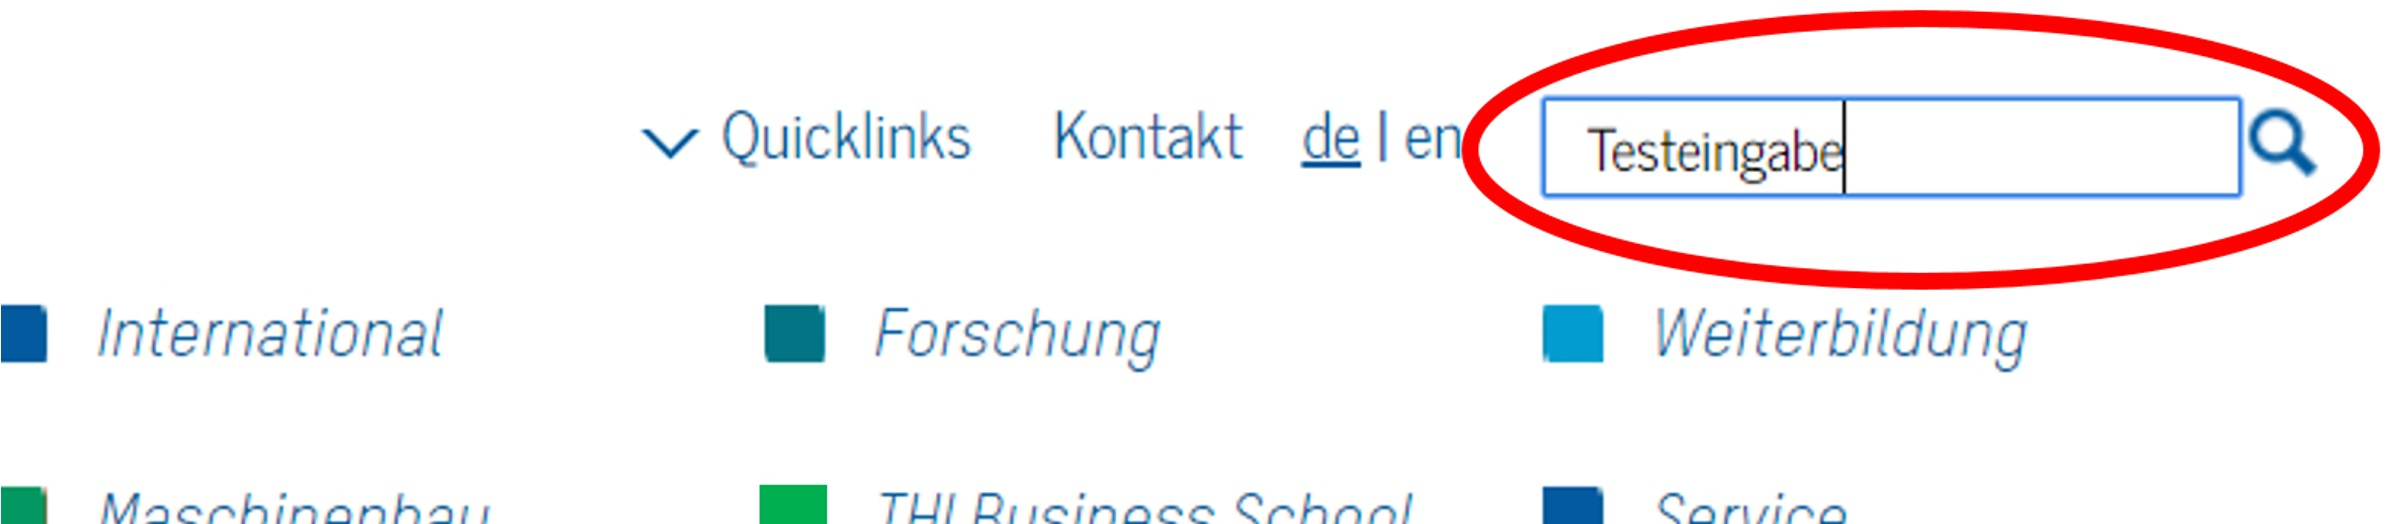
\includegraphics[width=0.9\textwidth]{images/XSS/Testeingabe_markiert.jpg}
	\caption{Eingabe eines Suchbegriffs}
	\label{fig:xss-reflected-Suche1}
\end{figure}

Das Ergebnis gibt in den meisten Fällen den eingegebenen Suchbegriff der Suche anschließend wieder aus. Dies ist auch in der Abbildung \ref{fig:xss-reflected-Suche2}  zusehen. So ergibt sich nun eine potentielle Angriffsstelle für einen Reflected Cross-Site-Scripting Angriff. Denn wenn man nun anstatt einer Texteingabe einen Scriptcode in das Suchfeld eingibt und dieser nicht überprüft wird, wird der Code beim anschließenden Ausgeben ausgeführt.\\

\begin{figure}[H]
	\centering
	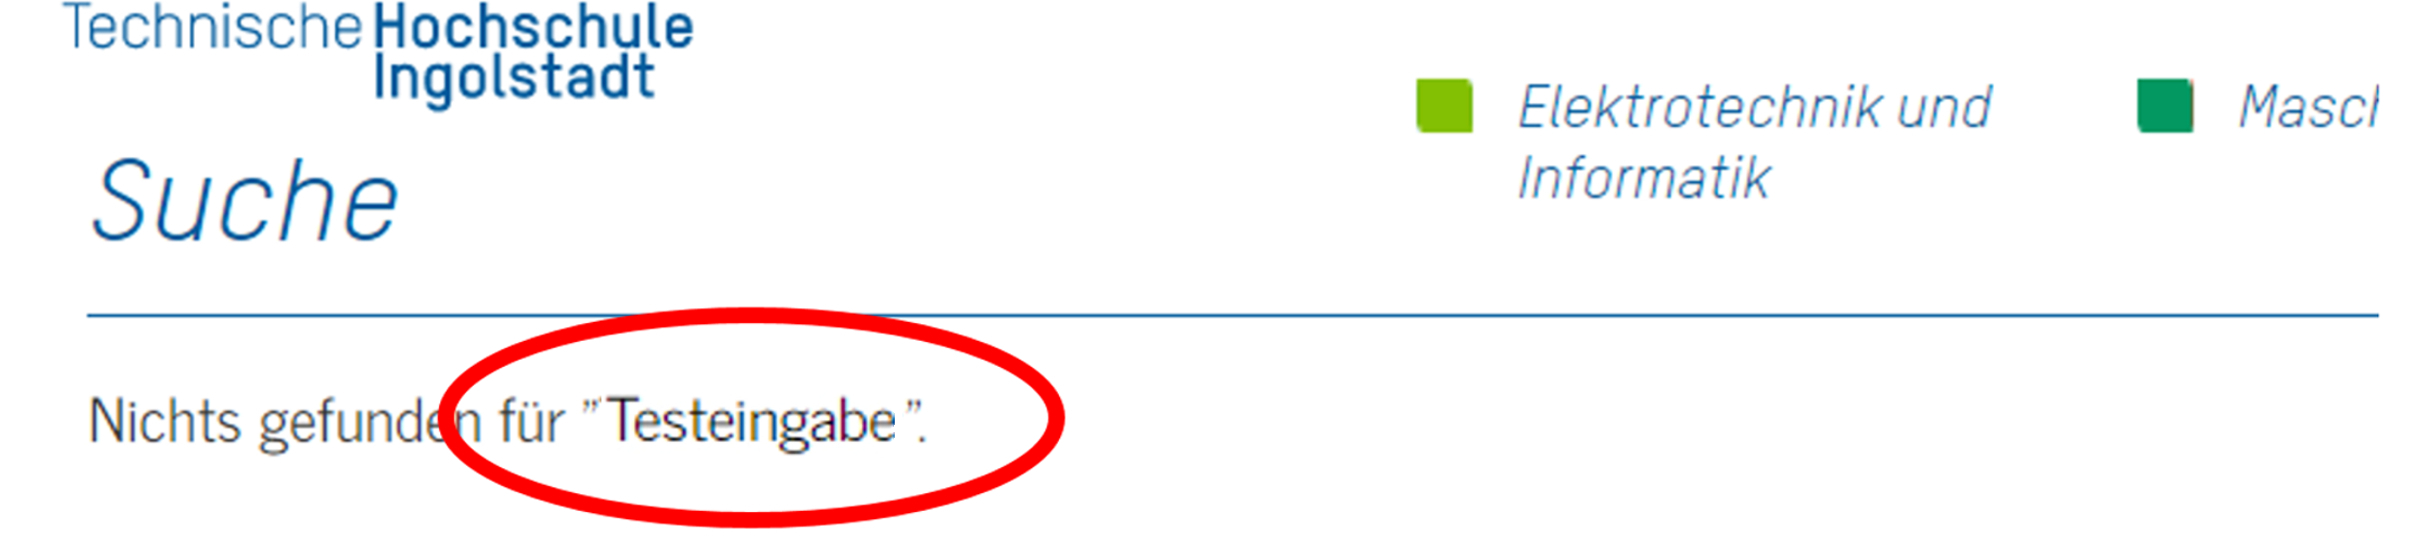
\includegraphics[width=0.9\textwidth]{images/XSS/Testergebnis_markiert.jpg}
	\caption{Ergebnis der Suche}
	\label{fig:xss-reflected-Suche2}
\end{figure}

Da die Benutzereingaben in den aktuellen Webanwendungen meistens überprüft werden, bietet nicht jede Webanwendung inkl. Suchfunktion eine Stelle für einen Reflected-XSS Angriff. 
Doch es finden sich immer wieder, auch in gängigen Webanwendungen, Sicherheitslücken, sodass ein Reflected-XSS Angriff mit vergleichsweise geringen Aufwand ausgeführt werden kann. \\
\ \\
\ \\
In der nachfolgenden Abbildung (\ref{fig:xss-reflected-grafik}) wird der Ablauf des Reflected-Cross-Site-Scripting Angriffs zur Verdeutlichung nochmals graphisch dargestellt.

\begin{figure}[H]
	\centering
	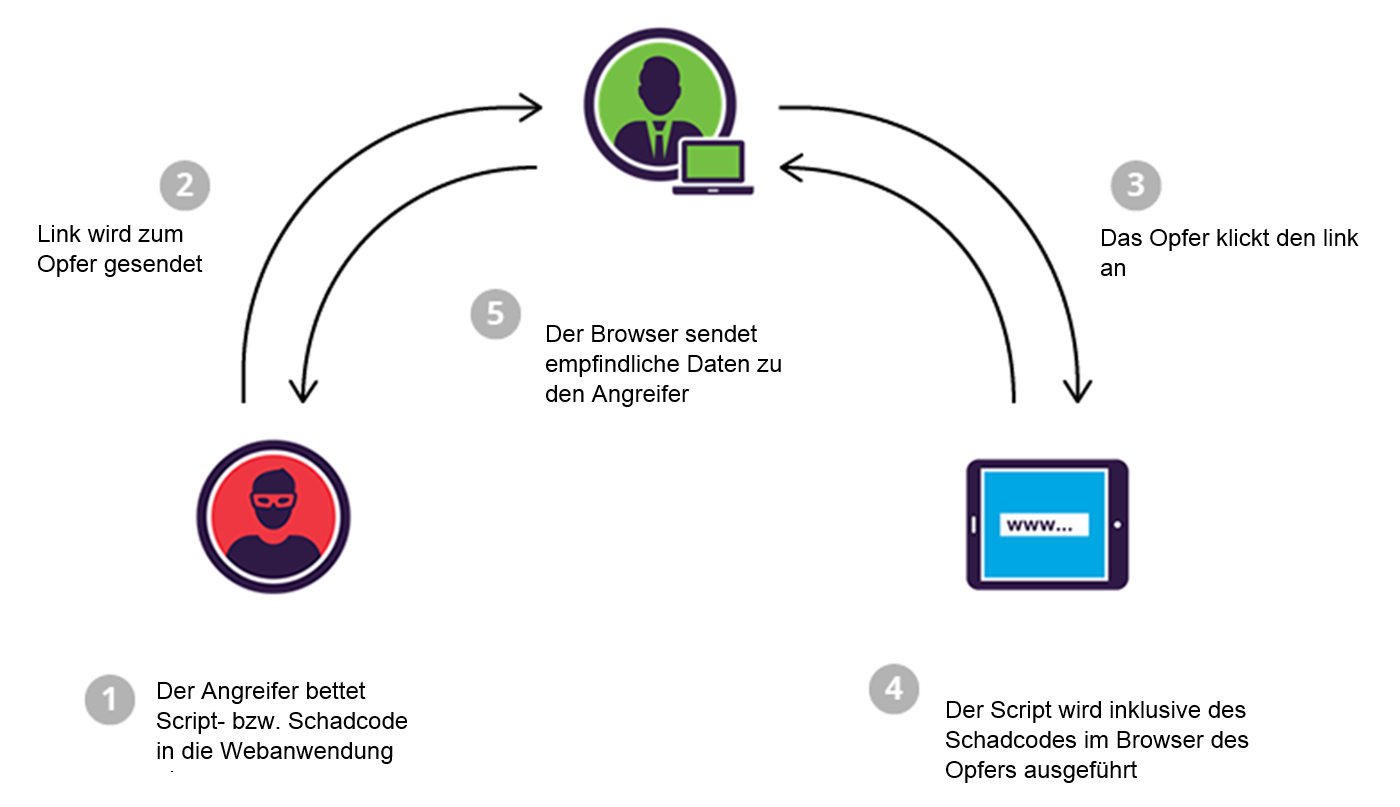
\includegraphics[width=\textwidth]{images/XSS/xss_reflected.png}
	\caption{Graphische Darstellung des Refelcted XSS-Angriffs}
	\label{fig:xss-reflected-grafik}
\end{figure}

\ \\
\ \\

\begin{wrapfigure}{r}{7.5cm}
  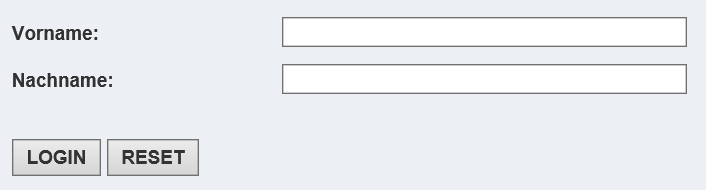
\includegraphics[width=7cm]{images/XSS/Anmeldeformular.jpg}
  \caption{Anmeldeformular}
\end{wrapfigure}
Bei den folgenden Übungen ist die Angriffsstelle nicht wie so oft die Suchfunktion, sondern ein Formular bei dem, der Benutzer Vor- und Nachname eingibt. 
Die Benutzereingaben werden nach dem betätigen des „LOGIN“-Buttons mit einer Grußformel ausgegeben, sodass der Benutzer mit seinem vollen Namen begrüßt wird. Dadurch, dass die Eingaben direkt wieder ausgegeben werden, bietet sich auch hier, wie im Fall der Suchfunktion, eine Angriffsstelle für Reflected-Cross-Site-Scripting. 
Im Gegensatz zu aktuellen Webanwendungen wurde es bei dieser, durch geringe bzw. keine Überprüfung der Benutzerdaten, erleichert einen Angriff zu fahren.
\newpage

\underline{1. Übung:}
\\
Bei der ersten Übung wird lediglich geprüft ob die Theorie hinter den Angriff gut verstanden wurde und prinzipiell anwendbar ist. Dazu soll man in eines der beiden Eingabefelder einen Scriptcode und in das andere Eingabefeld ein/e beliebiges Zeichen/folge eingeben, da beide Felder befüllt sein müssen bevor Vor- und Nachname ausgegeben werden können. Nachdem Betätigen des "`LOGIN"'-Buttons soll untenstehende Meldefenster (Abbildung\ref{fig:xss-reflected-DialogfensterI}) erscheinen.
\\
\\
Ein möglicher Scriptcode lautet:

\begin{figure}[h]
	\centering
	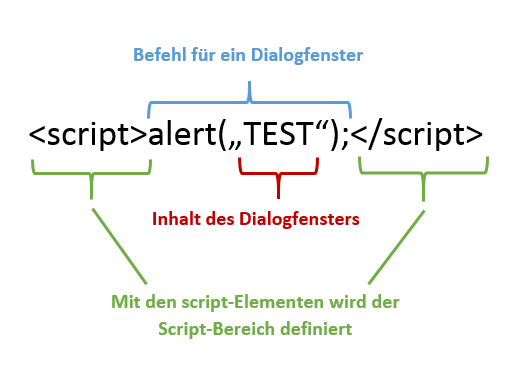
\includegraphics[scale = 0.4]{images/XSS/Scriptcode.jpg}
	\caption{Beispiel für einen Scriptcode}
	\label{fig:xss-reflected-Scriptcode}
\end{figure}

\ \\

\begin{figure}[h]
	\centering
	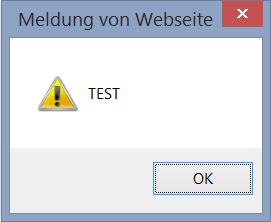
\includegraphics[scale = 0.4]{images/XSS/alert_meldung.jpg}
	\caption{Ausgabe des integrierten Scriptcodes}
	\label{fig:xss-reflected-DialogfensterI}
\end{figure}

\newpage

\underline{2. Übung:}
\\
Die zweite Übung unterscheidet sich nur geringfügig von der ersten, dabei besteht der geringe Unterschied in der Steigerung des Schwierigkeitsgrades. D.h. es werden bei dieser Übung die einfachen und die doppelten Anführungszeichen nicht mehr zugelassen.
Daraus folgt, dass der Scriptcode der 1. Übung nicht mehr funktioniert. Die Ausgabe bleibt dabei unverändert (Abbildung\ref{fig:xss-reflected-DialogfensterII})
\\
\\
Ein möglicher Scriptcode lautet daher: 

\begin{figure}[h]
	\centering
	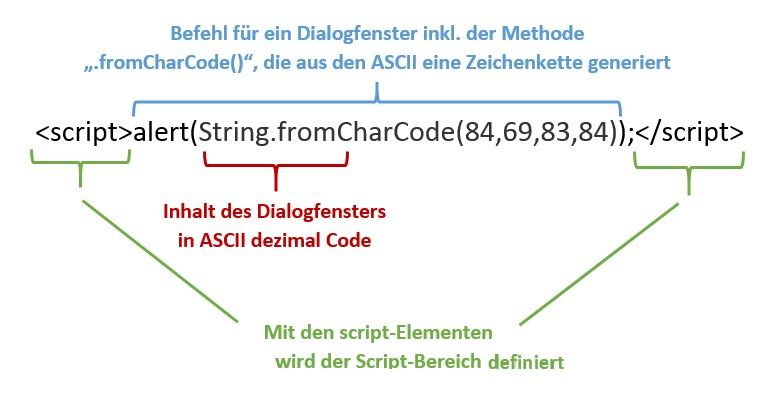
\includegraphics[scale = 0.4]{images/XSS/ScriptcodeII.jpg}
	\caption{Beispiel für einen Scriptcode}
	\label{fig:xss-reflected-ScriptcodeII}
\end{figure}

\ \\

\begin{figure}[h]
	\centering
	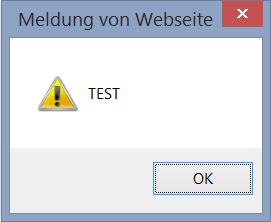
\includegraphics[scale = 0.4]{images/XSS/alert_meldung.jpg}
	\caption{Ausgabe des integrierten Scriptcodes}
	\label{fig:xss-reflected-DialogfensterII}
\end{figure}

\newpage

\underline{3. Übung:}
\\
Wie schon bei der zweiten Übung verändert sich hier nur der Schwierigkeitsgrad gegenüber der vorherigen Übung. 
Daraus ergibt sich das neben den einfachen und doppelten Anführungszeichen auch die Zeichenfolge "`script"' bei dieser 
Übung nicht mehr verwendet werden kann. Die Ausgabe bleibt wie schon in der 2. Übung unverändert (Abbildung\ref{fig:xss-reflected-DialogfensterIII}).
\ \\
\ \\
Ein möglicher Scriptcode lautet deshalb:

\begin{figure}[h]
	\centering
	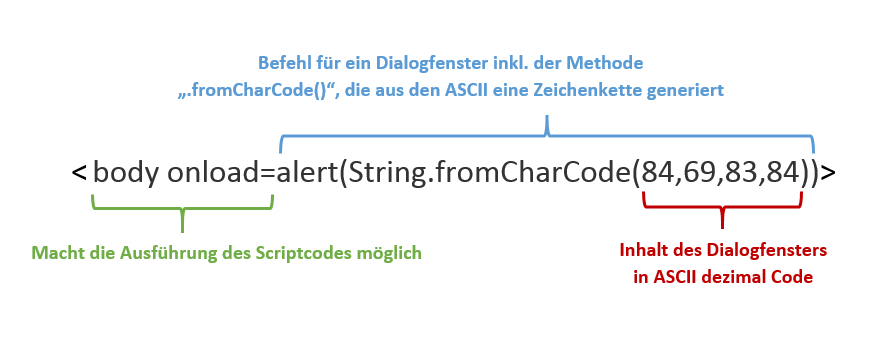
\includegraphics[scale = 0.4]{images/XSS/ScriptcodeIII.jpg}
	\caption{Beispiel für einen Scriptcode}
	\label{fig:xss-reflected-ScriptcodeIII}
\end{figure}

\ \\

\begin{figure}[h]
	\centering
	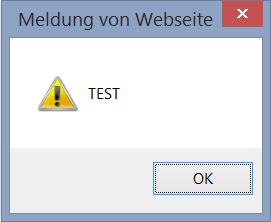
\includegraphics[scale = 0.4]{images/XSS/alert_meldung.jpg}
	\caption{Ausgabe des integrierten Scriptcodes}
	\label{fig:xss-reflected-DialogfensterIII}
\end{figure}

\newpage

\underline{4. Übung:}
\\
Nachdem die Übungen 1-3 das Verständnis und die Logik des Reflected Cross-Site-Scripting stärken sollen, sollen die kommenden Übungen ein praktisches Beispiel des Angriffs liefern.
Im Gegensatz zu den ersten Übungen, bei denen der Fremdcode auf dem eigenen Rechner ausgeführt wird und harmlos ist, soll nun ein möglicherweise schädlicher Code eingefügt und dessen Versendung behandelt werden.
So soll ein zweites Anmeldeformular eingebunden werden, das den Benutzer von seiner Korrektheit überzeugen soll, sodass er in dieses seine vertraulichen Daten eingibt.
Die Benutzerdaten werden anschließend Richtung Angfreifer gesendet.
\\
Ein möglicher Schadecode lautet:

\begin{figure}[h]
	\centering
	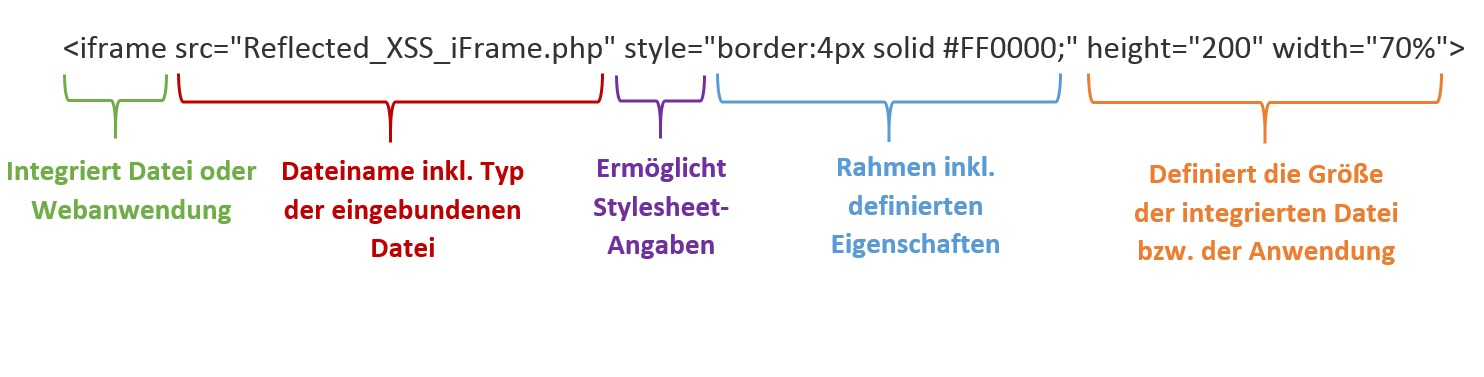
\includegraphics[width=\textwidth]{images/XSS/ScriptcodeIV.jpg}
	\caption{Beispiel für einen Scriptcode}
	\label{fig:xss-reflected-ScriptcodeIV}
\end{figure}

\ \\

\begin{figure}[h]
	\centering
	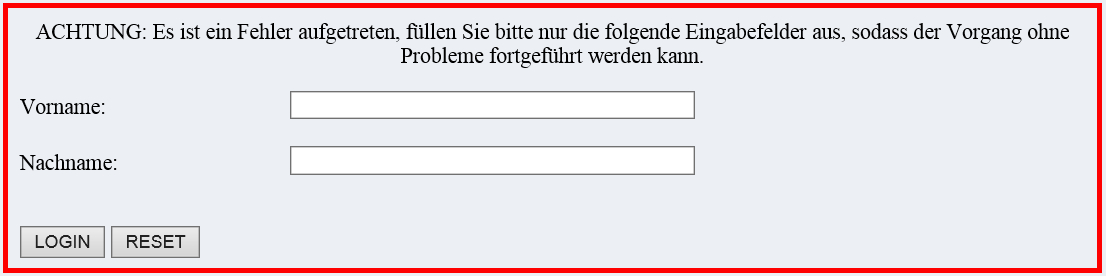
\includegraphics[width=\textwidth]{images/XSS/fremdes_anmeldeformular.jpg}
	\caption{Ausgabe des integrierten Scriptcodes}
	\label{fig:xss-reflected-ScriptcodeIV.1}
\end{figure}

Was man bei dieser und auch schon bei den vorangegangenen Übungen beobachten kann ist, das die Eingaben in den Eingabefelder, die normalerweise für Vor- und Nachname gedacht sind, nach den Betätigen des „LOGIN“-Buttons in der URL verankert ist. Daraus ergibt sich das der Schadcode mittels der URL versendet werden kann.

\newpage

\underline{5. Übung:}
\\
Die fünfte Übung ist der vierten sehr ähnlich. Lediglich der Schwierigkeitsgrad ist erhöht. 
D.h. einfache Anführungszeichen, doppelte Anführungszeichen und die Zeichenkette "`script"' sind bei dieser Aufgabe nicht zugelassen, alles andere bleibt gegenüber der vorherigen Übung gleich.
\\
Ein möglicher Schadecode lautet:

\begin{figure}[h]
	\centering
	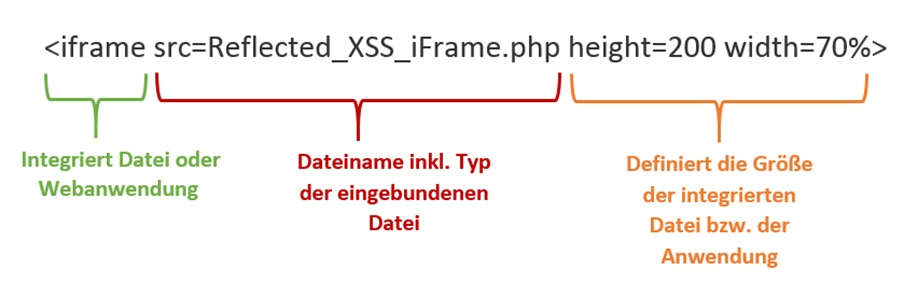
\includegraphics[width=\textwidth]{images/XSS/ScriptcodeV.jpg}
	\caption{Beispiel für einen Scriptcode}
	\label{fig:xss-reflected-ScriptcodeV}
\end{figure}

\ \\

\begin{figure}[h]
	\centering
	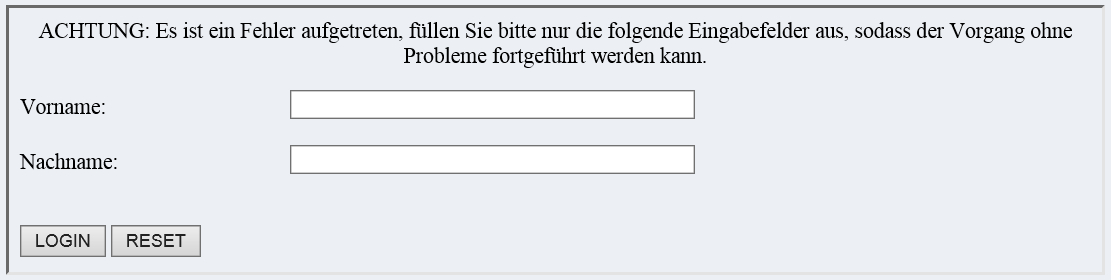
\includegraphics[width=\textwidth]{images/XSS/fremdes_anmeldeformular_II.jpg}
	\caption{Ausgabe des integrierten Scriptcodes}
	\label{fig:xss-reflected-ScriptcodeV.1}
\end{figure}
\ \\
Beim Vorgang des Versenden ändert sich nichts.

\newpage


\subsection{Stored Cross-Site-Scripting}
Im Tutorial für die Stored-XSS findet der Einsteiger ein Gästebuch wieder, dem Einträge hinzugefügt werden können. Hierzu sind diese mit einer Datenbank gekoppelt und werden dauerhaft gespeichert. Das Laden der Seite führt dazu, dass die Anwendung sich den Inhalt der Datenbank holt und in eine Tabelle schreibt. Um hier eine Sicherheitslücke zu schaffen werden die Usereingaben nicht überprüft und ungefiltert übermittelt. \\ 
Die Abbildung \ref{fig:stored-xss-aufgabe} zeigt das Gästebuch. Folglich soll der Einsteiger hier ein XSS-Angriff durchführen und die Cookies auslesen. In diesen sind die Credentials mit Username/ Passwort fälschlicherweise gespeichert. \\ 

\begin{figure}[H]
	\centering
	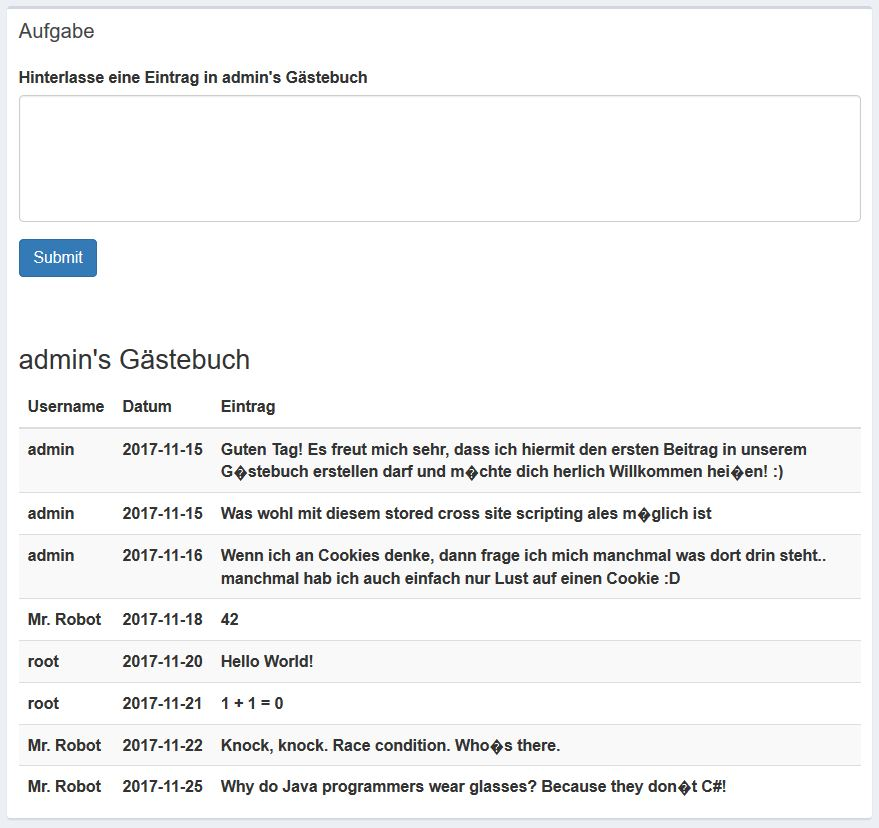
\includegraphics[width=\textwidth]{images/XSS/stored-xss-aufgabe.jpg}
	\caption{Darstellung des theoretischen Hintergrund für Stored-XSS}
	\label{fig:stored-xss-aufgabe}
\end{figure}

Die Lösung für das Tutorial ist es somit, dass der Einsteiger einen Gästebucheintrag verfasst, in dem ein Skript injiziert wird. Ein Beispiel hierfür ist \colorbox{altgray}{\lstinline|<script>alert("Hello World!");</script>|}. Da es für die Lösung der Aufgabe erforderlich ist die Cookies auszulesen, muss der Eintrag die folgende Zeichensequenz enthalten: 
\begin{center} 
\colorbox{altgray}{\lstinline|<script>alert(document.cookie);</script>|} 
\end{center}

Um den Einsteiger optimal auf die Übung vorzubereiten, besitzt dieses Tutorial ein Video mit dem theoretischen Hintergrund für Stored-XSS. Zudem werden dem Einsteiger Tipps an die Hand gegeben um die Aufgabe zu lösen. Abschließend ist zu erwähnen, dass auf dieser Tutorialseite auch die Gegenmaßnahmen dargestellt sind. Die Abbildung \ref{fig:stored-xss-theorie} veranschaulicht das eben Beschriebene. 

\begin{figure}[H]
	\centering
	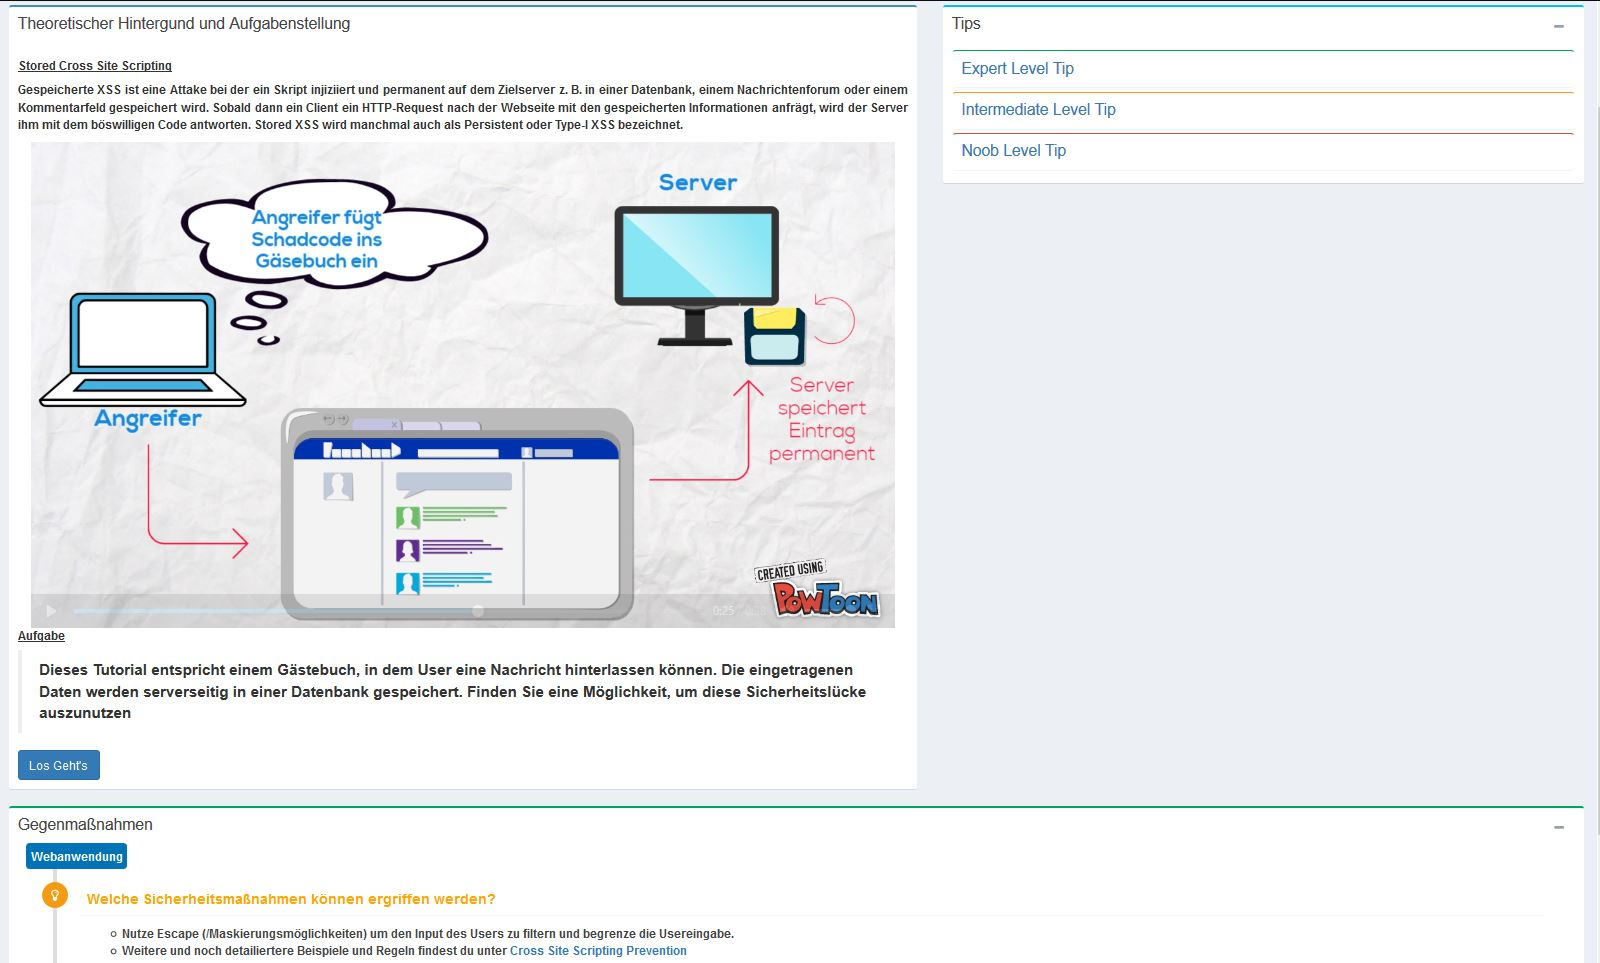
\includegraphics[width=\textwidth]{images/XSS/stored-xss-theorie.jpg}
	\caption{Darstellung des theoretischen Hintergrund für Stored-XSS}
	\label{fig:stored-xss-theorie}
\end{figure}

\subsection{DOM-Based Cross-Site-Scripting}
Das letzte Tutorial in Bezug auf XSS-Angriffe befasst sich mit der Variante des DOM-Based-XSS. Hierzu wurde exemplarisch eine Sprachauswahl implementiert, bei der eine Selektierungsmöglichkeit über die URL erzeugt wird. Das folgende Listing \ref{lstlisting:Select-DOM-based} zeigt diesen Anwendungskontext: 
\begin{lstlisting}[caption=Select-Statement\label{lstlisting:Select-DOM-based}]{Name}
<select id="languageList" style='width:500px'>
	<script>
	document.write("<OPTION value=1>" + 				document.location.href.substring(document.location.href.indexOf("default=") + 8) + "</OPTION>");
	</script>
</select>
\end{lstlisting}
Hier wird eine Select-Option über JavaScript erzeugt, indem auf die URL zugegriffen wird. Die Default URL für dieses Tutorial ist \\ \colorbox{altgray}{\lstinline|http://localhost/html/DOMbasedXSS.html?default=german|}. Folglich entspricht eine Auswahlmöglich der Sprache \textit{german}, die restlichen Wahlmöglichkeiten werden über JavaScript inkludiert. Die Abbildung \ref{fig:dom-based-xss-aufgabe} zeigt die Aufgabenstellung. 
\begin{figure}[H]
	\centering
	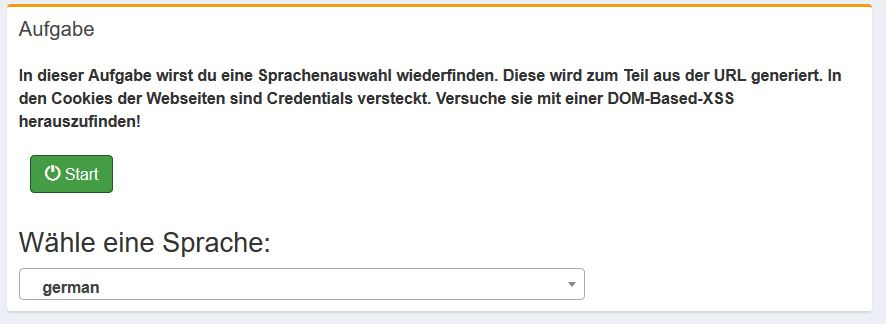
\includegraphics[width=\textwidth]{images/XSS/dom-based-xss-aufgabe.jpg}
	\caption{Aufgabenstellung des DOM-based-XSS Tutorials}
	\label{fig:dom-based-xss-aufgabe}
\end{figure}
Um das Tutorial zu lösen muss der Einsteiger die URL manipulieren, indem er dort ein Skript in die Anwendung injiziert. Hierzu soll der erneut die Cookies auslesen. Die Lösung für das Tutorial ist somit: 
\begin{center} 
\colorbox{altgray}{\lstinline|.../DOMbasedXSS.html?default=german<script>alert(document.cookie);</script>|} 
\end{center}
Wichtig ist es bei diesem Tutorial auf die Sicherheitseinstellungen des Browsers zu achten. So werden z. B. unter Firefox die Eingaben in der URL gefiltert, sodass es nicht möglich ist ein Script zu übergeben. Hingegen bieten einige Versionen des Internet Explorer diesen Schutz noch nicht. Daher sollten die Einsteiger entweder versuchen die Schutzmechanismen des Browser zu deaktivieren oder einen unsicheren Browser verwenden. \\ 
Abschließend muss hier erwähnt werden, dass auch dieses Tutorial ein Theorievideo sowie Tipps und Gegenmaßnahmen besitzt. 





